\documentclass{article}
\usepackage{url,epsfig,capt-of}
%\nonstopmode
\def\DensiTree{DensiTree}
\def\webdir{/Users/remco/research/DensiTree/web}

\title{\DensiTree\ Manual: \\{Making sense of sets of trees}\\Version 2.2}
\author{Remco Bouckaert\\
\url{r.bouckaert@auckland.ac.nz}\\
%\url{remco@cs.waikato.ac.nz}\\
%\url{rrb@xm.co.nz}
}

\setcounter{tocdepth}{1}
\begin{document}
\maketitle
\newpage
\tableofcontents
\newpage


\section{Introduction}

Bayesian hierarchical clustering methods provide a powerful tool for phylogenetic 
analysis, linguistic research and hierarchical clustering in general such as applied
in marketing, political science, customer preference grouping etc.
One of the benefits of the Bayesian approach over classical hierarchical clustering
methods such as single-link, complete link and Ward clustering is that it provides
a measure of the lengths of the branches in the hierarchy. A further benefit over
maximum likelihood clustering is that the Bayesian method provides insight in the 
distribution of possible hierarchies.
Bayesian methods use MCMC sampling which results in a large number of trees
representing the distribution over all possible hierarchies.
Unfortunately, interpreting this distribution is not straight forward since
the set of trees produced by an MCMC analysis can run in the thousands
and examining them individually would be too laborious.

A popular method for analyzing tree sets are to find a single representative
hierarchy and label the branches with uncertainty (for instance using the
TreeLogAnnotator in BEAST \cite{BEAST}). The benefit of this method is that it is 
easy to interpret the single hierarchy by visualizing it in a tree drawing program
(such as FigTree \cite{FigTree}) and use error bars to indicate uncertainty in 
branch lengths. Unfortunately, it takes some skill to interpret situations
where there is uncertainty in the hierarchy. Such cases show in the tree
as short branches with relatively large error bars. However, this is indistinguishable
from the case where a single tree topology dominates but where there is large 
uncertainty due to model and/or data.

Another method for interpreting tree sets is to find subtrees (aka clades) that
occur with high frequency (for example by using the TreeLogAnalyser in BEAST 
\cite{BEAST}). The number of relevant clades may become very large, especially
with large datasets since the number of possible trees grows exponentially
in the number of labels. Furthermore, interpreting uncertainty within high
frequency clade may become cumbersome due to the large number of them.

Tree networks (as in SplitsTree \cite{SplitsTree}) are graphs containing
edges wherever such edges appear (possibly at some threshold frequency)
in the tree set. Tree networks do not allow easy representation of
uncertainty %(CHECK!!!) 
and can become unwieldy when large numbers of
distinct topologies are present in the tree set.

Here, we provide an alternative method for tree set analysis implemented
in an open source tool \DensiTree\ freely available under GPL license.
\DensiTree\ is a program for drawing sets of trees stored in Nexus format.
The main idea is to draw all trees in the set, but instead of using opaque
lines, we use transparency. As a result, areas where a lot of the trees agree
on the topology and branch length, there will be many lines drawn and the
screen will show a densely colored area. Areas where there are a few competing
topologies will be highlighted by a web of lines.
Uncertainty in node heights and their distribution can be shown by smears
around the mean node height.
Where summary trees and clade sets are quantitative approaches to tree set analysis,
\DensiTree\ provided a qualitative approach.

We start with some important concepts for understanding \DensiTree\ in Section \ref{ssec.cpt}.
The main features and analysis methods that can be performed with \DensiTree\ are
shown in the gallery (Section \ref{sec.gal}). The user 
interface is explained in Section \ref{sec.gui}, including the menu items
and table of key short cuts. 
Section \ref{sec.faq} is called FAQ and lists some common things one may want to do.
Finally, command line interface is described in 
Section \ref{sec.cmd}, which is useful for starting \DensiTree\ with your
favorite standard settings.

\subsection{Important concepts \label{ssec.cpt}}

The complete set of trees represented in the NEXUS file will be referred to
as the {\em set of all trees}.

The set of all trees has a limited number of topologies. For every topology,
a so called {\em consensus tree} is calculated. The branch length of a consensus
tree is calculated as the average of the branch length for all trees with the
same topology. So, there are two sets of trees in \DensiTree, a set of all trees
and a set of consensus trees. Both can be drawn or either of them can be drawn.

There are two ways of viewing; the default is {\em draw all} which draws the set 
of trees and/or consensus trees. Alternatively, one can {\em browse} through the
tree topologies.

\subsection{What is new \label{ssec.new}}
From Version 2.1 to 2.2, the following changes were made:

o support for images as labels

o more robust geography data parsing

o allow geography draw lines from the left

o better integration with summary\_tree

o support for .densitree configuration file with default settings

o many small bugs

From Version 2.01 to 2.1.10, the following changes were made:

o layout improved

o burn-in by percentage, default to 10\%

o ability to hide labels

o tip tools

o user specified root canal tree

From Version 2.0 to 2.01, the following changes were made:

o Star tree, centralised tree and angle correction added.

o Button bar with tree type/style.

o List of clades, select clade by clicking in the list.

o Interactive clade movement.

o Numerics: better scales, height tracking of cursor, cumulative tree intensity reported when browsing, view clade support percentage

From Version 1.45 to 2.0, the following changes were made:

o Edit tree to manipulate rotation and height of internal nodes.

o Support of phylogeographical images.

o A choice of branch drawing methods (lines, arcs, steep arcs).

o Editing of trees be deleting taxa and saving resulting tree set.

o Pasting trees from clipboard.

o Label rotatable when the root is at top + more sensible label placement.

\newpage
\section{Getting started\label{sec.start}}

To run \DensiTree, you need a Java at least version 6 runtime installed (but version 7 or higher is faster). This is available for instance available from \url{http://java.com}). You also need the \DensiTree\ binary,
which can be downloaded from \url{http://www.cs.auckland.ac.nz/~remco/DensiTree}.

You can run \DensiTree\ by calling {\tt java -jar DensiTree.jar} from the command line. Make sure that the file DensiTree.jar is in the directory you start at.

Sorry, it's not more complex than this.

\newpage
\section{Gallery\label{sec.gal}}

This section shows the main features of \DensiTree\ and highlights some of the
methods useful for interpreting tree sets.

\begin{center}
\includegraphics[width=\textwidth]{\webdir/mcc.png}
\captionof{figure}{\label{fig.mcc}Default setting when opening a file.
Show both consensus trees and set of all trees in triangular shape. 
In this tree set, there are five clearly distinguishable clades, with
large uncertainty of the topologies within the two 5-leaf clades.
}
\end{center}

\newpage
\begin{center}
\includegraphics[width=\textwidth]{\webdir/mcmc.png}
\captionof{figure}{\label{fig.mcmc}
Show only consensus trees. This set shows that
there is very little uncertainty in the topology of most of the tree, except for
the few splits near the root.
}
\end{center}

\newpage
\begin{center}
\includegraphics[width=\textwidth]{\webdir/votes.png}
\captionof{figure}{\label{fig.nzvotes}
Show only consensus trees. This highlights the uncertainty inside the clades, but
shows that the split at the root into two groups is very certain (split into
progressive and conservative politicians).
}
\end{center}


\newpage
\begin{center}
\includegraphics[width=\textwidth]{\webdir/mayan3.png}
\captionof{figure}{\label{fig.mayanheight}Show tree height by height grid and height bar.
This tree set nicely demonstrates the increase in uncertainty of the node heights going from
the leafs to the root.}
\end{center}

\newpage
\begin{center}
\includegraphics[width=\textwidth]{\webdir/mayanblock.png}
\captionof{figure}{\label{fig.mayanblock}As Figure \ref{fig.mayanheight} but in block trees.
This tree set was generated with calibration points, which show up as dense node heights,
for example, the parent of Rrr and Bbb.}
\end{center}

%\newpage
%\begin{center}
%\includegraphics[width=\textwidth]{\webdir/mayanlog.png}
%\captionof{figure}{\label{fig.mayanlog}Using log scale for height. This can be helpful
%for tree sets with very long root branches and short leaf branches. Note that \DensiTree\ uses
%$log(h+1)$ where $h$ is the node height, so when the absolute branch lengths are close to zero
%then $log(h+1)$ is close to $h$ and almost no gain in visibility is made.}
%\end{center}


\newpage
\begin{center}
\includegraphics[width=\textwidth]{\webdir/virus.png}
\captionof{figure}{\label{fig.virus}Decreased width of consensus trees, only consensus trees drawn.
Intensity of consensus trees needed to be increased considerably.
This is useful when there is large uncertainty in the topology and hence many consensus trees (over 900
in this example) with little overlap. Without intensity increase they would not show up and only a
white image would be shown.}
\end{center}

%\begin{center}
%\includegraphics[width=\textwidth]{\webdir/ourisia.png}
%\captionof{figure}{\label{fig.ourisia}Root at top}
%\end{center}

\newpage
\begin{center}
\includegraphics[width=\textwidth]{\webdir/ourisia2.png}
\captionof{figure}{\label{fig.ourisia2}Triangle tree with root at top.
This can be an attractive option when there are not a lot of leafs so that
the labels do not overlap.}
\end{center}

\newpage
\begin{center}
\includegraphics[width=\textwidth]{\webdir/ourisia3.png}
\captionof{figure}{\label{fig.ourisia3}Increase intensity consensus trees.
Consensus trees are drawn with intensity proportional to the frequency of 
occurrence of the topology in the set. As a result, low frequency topologies
will be drawn very faintly and may become invisible. By increasing the 
global intensity, these faint trees can be made more visible.
}
\end{center}

\begin{center}
\includegraphics[width=\textwidth,height=8cm]{\webdir/ourisianojitter.png}
\includegraphics[width=\textwidth,height=8cm]{\webdir/ourisia4.png}
\captionof{figure}{\label{fig.ourisia4}Jitter x-axis.
Especially the block-layout of a tree results in many overlapping lines in the
direction from the leafs to the root. These show up as dense stripes in the
image (see top image). By adding jitter to the begin and end points, the lines 
get randomly perturbed with a small amount and the image gives a better sense 
of the densities (bottom image).}
\end{center}


\begin{center}
\includegraphics[width=\textwidth,height=8cm]{\webdir/poly4.png}
\includegraphics[width=\textwidth,height=8cm]{\webdir/poly3.png}
\captionof{figure}{\label{fig.poly3}Move leaf for better layout on Polynesian language data \cite{poly}.
In this case, the leaf at 
the top is moved to the bottom, resulting in the long branch to that leaf being shortened 
considerably. In situations where there is a lot of uncertainty in the topology near the
leafs it is often possible to move a few leafs a bit to minimize the number of crossing
lines and get a clearer view.}
\end{center}

\begin{center}
\includegraphics[width=\textwidth]{\webdir/poly.png}
\captionof{figure}{\label{fig.poly}Zoom in (Data from  \cite{poly}).}
\end{center}


\begin{center}
\includegraphics[width=\textwidth]{\webdir/poly2.png}
\captionof{figure}{\label{fig.poly2}Draw trees up from selected leafs.
Only tree branches with a direct path from the root to a selected
leaf will be drawn.  Data from  \cite{poly}.}
\end{center}



\begin{center}
\begin{tabular}{cc}
\includegraphics[width=0.5\linewidth]{\webdir/ourisia5.png} & \includegraphics[width=0.5\linewidth]{\webdir/ourisia6.png} \\
\includegraphics[width=0.5\linewidth]{\webdir/ourisia7.png} & \includegraphics[width=0.5\linewidth]{\webdir/ourisia8.png} \\
\end{tabular}
\captionof{figure}{\label{fig.ourisia5}Show selection of tree topologies.
Top left shows the most likely tree topology, and the consensus tree with that topology
drawn in. Top right shows the second most popular topology. Bottom left the third most
likely. Bottom right shows the second and third most likely tree topologies, leaving
out the most likely topology.}
\end{center}


\begin{center}
\includegraphics[width=8cm]{\webdir/ourisia9.png}
\captionof{figure}{\label{fig.ourisia9}Not recommended, but possible:
an example of color and font customization. Here, font size is increased
to 48 point, color of all trees set to red, color of consensus trees to green
and background color to yellowish green.
}
\end{center}

\begin{center}
\includegraphics[width=5cm]{\webdir/bulgaria.png}
\includegraphics[width=5cm]{\webdir/bulgaria2.png}
\captionof{figure}{\label{fig.bulgaria}When there are many topologies, each occurring
with low frequency, the result may be a mess (left image) because the order of leafs is chosen based on the
most frequently occurring consensus tree. To untangle the mess, various shuffle methods are
available under the Edit/Shuffle submenu (result in right image).
}
\end{center}

\begin{center}
\includegraphics[width=6cm]{\webdir/edittree.png}
\includegraphics[width=6cm]{\webdir/edittree2.png}
\captionof{figure}{\label{fig.edittree}When edit-tree is shown (through menu Edit/Show edit tree)
the order of taxa can be manipulated by clicking on the rotation icons drawn on the internal nodes
of the black tree.
}
\end{center}

\begin{center}
\includegraphics[width=\textwidth]{\webdir/phylogeography.png}
\captionof{figure}{\label{fig.phylogeography}
Phylogeographical DensTree where the taxa are connected with their geographical locations
and a background image showing a relevant map.
}
\end{center}

\begin{center}
\includegraphics[width=0.9\textwidth]{\webdir/metadata.png}
\captionof{figure}{\label{fig.metadata}
Drawing metadata embedded in the tree set to determine the y-position of the internal
nodes. Black dots at the 90\% highest probability density interval and the median.
}
\end{center}

\begin{center}
\includegraphics[width=0.9\textwidth]{\webdir/arc.png}
\includegraphics[width=0.9\textwidth]{\webdir/steeparc.png}
\captionof{figure}{\label{fig.arc}
Different methods of drawing branches. Arcs at the top, steep arcs at the bottom.
}
\end{center}

\newpage
\section{GUI\label{sec.gui}}\

When opening \DensiTree\ the following screen appears with a main window containing
a menu, tool bar, status bar.
\begin{center}
\includegraphics[width=\textwidth]{screenshots/densitree.png}
\captionof{figure}{\label{fig.overview}Main window}
\end{center}


\subsection{Menu items}
\DensiTree\ has the following menu items and short description of its function.

\begin{center}
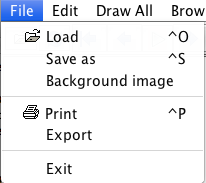
\includegraphics[width=4cm]{menufile.png}
\captionof{figure}{\label{fig.menufile}File menu}
\end{center}

\noindent
{\tt File/Load}: open Nexus trees file containing set of trees\\
{\tt File/Save as}: Save current tree set as Nexus tree file. Only useful after editing taxa in the tree\\
{\tt File/Background image}: open bitmap file to be shown in the background. If a KML file is
loaded, this is considered to be a world map, and only part of the image relevant to the locations
of the taxa is shown. If the KML file has a file name of the form "XYZ($<$lat1$>$,$<$long1$>$)x($<$lat2$>$,$<$long2$>$).png"
for example "NewZealand(-60,140)x(-10,180).png"
then the image is considered to cover only the rectangle with corners  ($<$lat1$>$,$<$long1$>$) and 
($<$lat2$>$,$<$long2$>$). Not lat1 $<$ lat2 and long1 $<$ long2.\\
{\tt File/Print}: print currently shown view of the tree set (untested)\\
{\tt File/Export}: export currently shown view of the tree set in bitmap in BMP, JPG, PNG and SVG
format.
Note that the zoom factor (menu {\tt Window/Zoom in} and {\tt .. out}) has impact on the resolution 
of the image. For hight resolution images, zoom in more, then redraw, then export.\\
{\tt File/Exit}: quit \DensiTree.

\begin{center}
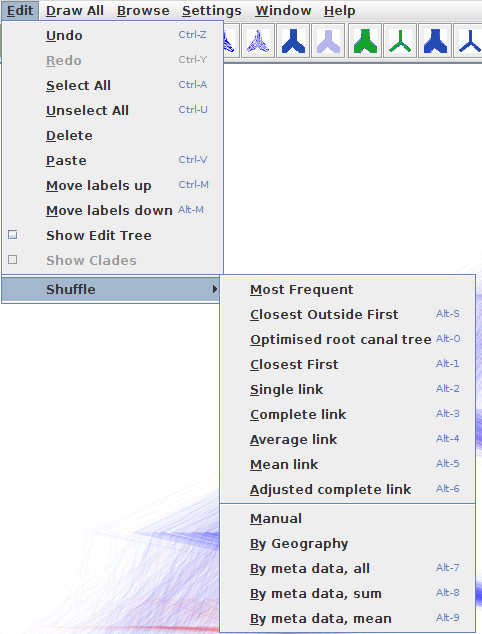
\includegraphics[width=4cm]{menuedit.png}
\captionof{figure}{\label{fig.menuedit}Edit menu}
\end{center}

\noindent
{\tt Edit/Undo}: undo latest reordering of taxa. Note that the undo action only applies
to reorderings, not to font changes, intensity settings, layout options, etc.\\
{\tt Edit/Redo}: redo latest reordering of taxa.\\
{\tt Edit/Select All}: select all leafs in the tree. This is useful when after manipulating
the order of the leafs a redraw is required with branches to all leafs shown.\\
{\tt Edit/Unselect All}: remove all leafs from selection. This is useful before moving a single
node.\\
{\tt Edit/Delete taxa}: remove selected taxa from tree. Branches between a taxon and its parent
will be removed one by one and the internal parent node removed.\\
{\tt Edit/Paste trees}: paste one or more trees in Nexus format from the clipboard.\\
{\tt Edit/Move labels up}: move selected labels one higher in the ordering. It is recommended to
use the short cut key {\tt Ctrl-M} if a large number of moves need to be made\\
{\tt Edit/Move labels down}: move selected labels one lower in the ordering. It is recommended to
use the short cut key {\tt M} if a large number of moves need to be made\\
{\tt Edit/Show Edit Tree}: Show a tree to allow reording of nodes by selecting the rotate icons
drawn on the internal nodes (see Figure \ref{fig.edittree}.\\
{\tt Edit/Show Clades}: Show a clades by drawing a circle with a radius proportional to its
support. This allows clades to be moved when drawing a centralised tree.\\
{\tt Edit/Shuffle}: Submenu with various methods for ordering the nodes.\\
{\tt Edit/Shuffle/Most Frequent}: Use order that displays most frequently occurring tree nicely. 
This is the default used when opening a file.\\
{\tt Edit/Shuffle/Closest First}: Orders leafs by starting with the closest two leafs, then
adding the closest node to the left most or right most node. The distance measure used is
based on the length of the edges averaged over all trees.\\
{\tt Edit/Shuffle/Single link}: Use single link hierarchical clustering with the distance method
as for 'closest first' and use an order that displays the obtained hierarchy pleasingly.\\
{\tt Edit/Shuffle/Complete link}: As single link, but using complete link.\\
{\tt Edit/Shuffle/Average link}: As single link, but using average link.\\
{\tt Edit/Shuffle/Mean link}: As single link, but using mean link.\\
{\tt Edit/Shuffle/Adjusted complete link}: As single link, but using adjusted complete link.\\
{\tt Edit/Shuffle/Manual}: Key in order of nodes by hand.\\
{\tt Edit/Shuffle/By Geography}: Only useful when geographic locations are loaded for the taxa.
Orders nodes by longitude if root at top, or latitude otherwise.\\
{\tt Edit/Shuffle/By meta data, all}: if meta data is available matching a pattern (can be
provided with the -pattern command line option) the tree is draw with internal nodes at
the level of the meta data value.\\
{\tt Edit/Shuffle/By meta data, sum}: as above but the sum of values at each height in the
tree is used as level.\\
{\tt Edit/Shuffle/By meta data, mean}: as above but mean value at each height is used.\\


\begin{center}
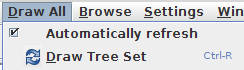
\includegraphics[width=4cm]{menudrawall.png}
\captionof{figure}{\label{fig.menuedrawall}Draw all menu}
\end{center}

\noindent
{\tt Draw all/Automatic refresh}: when selected, the tree set will be redrawn whenever a setting
changes. If not selected, an explicit redraw needs to be done (using short cut key {\tt R} or 
menu {\tt Draw all/Draw Tree Set}) to draw the tree set after manipulating some settings.\\
{\tt Draw all/Draw Tree Set}: draw tree set when automatic refresh is off, and switches to
drawing mode when in browsing or animation mode.


\begin{center}
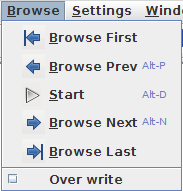
\includegraphics[width=4cm]{menubrowse.png}
\captionof{figure}{\label{fig.menubrowse}Browse menu}
\end{center}

\noindent
{\tt Browse/Browse First}: Shows first consensus tree and/or accompanying trees from set of
all trees. If in drawing mode, switch to browse mode. If in animation mode, animation is
stopped.\\
{\tt Browse/Browse Previous}: Show previous consensus tree. If it is the first tree,
or in over write mode (see menu {\tt Browse/Overwrite}), the screen is cleared before
drawing the tree set. Otherwise, the trees are drawn over already drawn trees.\\
{\tt Browse/Start}: Start/stop animation.\\
{\tt Browse/Browse Next}: Show next consensus tree. If in over write mode 
(see menu {\tt Browse/Overwrite}), the screen is cleared before drawing the tree set.
Otherwise, the trees are drawn over already drawn trees.\\
{\tt Browse/Browse Last}: Shows last consensus tree, clearing the screen if required.\\
{\tt Browse/Overwrite}: When not set (default) the trees are drawn on top of each other
when browsing the trees. This way, a subset of tree topologies can be drawn. 
If set, the screen is cleared and only a single topology is drawn when browsing or
animating.\\


\begin{center}
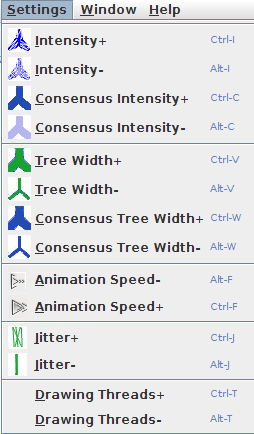
\includegraphics[width=6cm]{menusettings.png}
\captionof{figure}{\label{fig.menusettings}Settings menu}
\end{center}

\if0
\noindent
{\tt Settings/Show consensus trees}: Toggle to indicate whether consensus trees 
should be drawn.\\
{\tt Settings/Show all trees}: Toggle to indicate set of all trees should be drawn.\\
{\tt Settings/Show Root Canal}: Draw consensus tree with the highest clade support, which shows
up as a root canal.\\
{\tt Settings/Show root at top}: Toggle to have root at top and leafs at bottom, or
root on left and leafs on right.\\
%

\noindent
{\tt Settings/Method} Choose method for drawing a tree\\
{\tt Settings/Method/Default} Positions a node in the middle of the top of its two child clades.\\
{\tt Settings/Method/Star tree} Star trees point branches to the top of the tree.\\
{\tt Settings/Method/Centralised tree} Position a node in the middle of the extreme taxa of a clade.\\
{\tt Settings/Method/Centralised angle corrected} As centralised, but depending on a threshold, child clades
are positioned the same as their parent clade if the parent clade has 100\% support, but the child clades
less.\\
{\tt Settings/Method/Angle Correction +} Increase threshold for angle correction.\\
{\tt Settings/Method/Angle Correction -} Decrease threshold for angle correction.\\

\noindent
{\tt Settings/Style/Triangle} Use triangles for drawing a tree\\
{\tt Settings/Style/Block} Use block tree\\
{\tt Settings/Style/Arc} Use arc tree\\
{\tt Settings/Style/Steep arc} Use steep arcs for drawing a tree\\

\noindent
{\tt Settings/Show grid} Choose method for drawing a scale.\\
{\tt Settings/Show grid/No grid} Omit scale.\\
{\tt Settings/Show grid/Short grid} Show scale, but no lines through the trees.\\
{\tt Settings/Show grid/Full grid} Show scale and lines through trees.\\

\noindent
{\tt Settings/Meta data/Use meta data for line width} draw line where the width is determined by some meta data item.\\
{\tt Settings/Meta data/Pattern} Specify which meta data item is used for line width.\\
{\tt Settings/Meta data/Meta data scale} Scales line width. If the scale is not set properly, very thick lines or uninformative small lines are produced.\\
{\tt Settings/Meta data/Correct top of branch} If this flag is set, the top of the line is adjusted so that two coalescing branches fit the bottom of the following branche.\\

\noindent
{\tt Settings/Geography/Show Geo info}: Whether to draw lines from taxa to their geographical location.\\
{\tt Settings/Geography/Load locations}: open file with geographic location information of the taxa stored in
KML file which can be produced by Google earth.\\
{\tt Settings/Geography/Geo line widht}: Width of the line used to link taxon with its geographical location.\\
{\tt Settings/Geography/Geo color}: set color of the link between taxa and their geographical locations.\\

\noindent
{\tt Settings/Label/Set font}: set font properties (size, family. etc) of labels and height bar label.\\
{\tt Settings/Label/Label color}: set color of leaf labels.\\
{\tt Settings/Label/Label width}: changes the width of the labels (default 100) when drawn with root at left.\\
{\tt Settings/Label/Rotate labels}: whether to rotate labels when the root is draw at the top.\\

\noindent
{\tt Settings/Line Color/Multi color consensus trees}: when selected, consensus trees are drawn using 18 different colors
instead of the single default color.\\
{\tt Settings/Line Color/Color 1 .. 3}: set color of most popular tree topology, second most popular and third most popular tree topology.
{\tt Settings/Line Color/Default color}: set color of remaining tree topologies.\\
{\tt Settings/Line Color/Consensus color}: set color of consensus trees.\\
{\tt Settings/Line Color/Background color}: set background color.\\
{\tt Settings/Line Color/Root canal color}: set color of the root canal tree.\\
%
%{\tt Settings/Use log scale for Height}: Toggle between using heights from the 
%Nexus trees file or using $\log(height+1)$ instead. This can be useful when the
%majority of branches split close to the leafs.\\
%{\tt Settings/Show height grid}: show height lines across image splitting the
%largest height in 10 equally sized intervals.\\
%{\tt Settings/Show height bar}: show bar indicating 1/10th of height with
%label of its size.\\
\fi

\noindent
{\tt Settings/Intensity- and +}: decrease/increase tree intensity.\\
{\tt Settings/Consensus Intensity- and +}: decrease/increase consensus tree intensity.\\
{\tt Settings/Tree width- and +}: decrease/increase tree line width.\\
{\tt Settings/Consensus Tree width- and +}: decrease/increase consensus tree line width.\\
{\tt Settings/Animation speed- and +}: decrease/increase animation time delay - shorter delay = faster animation.\\
{\tt Settings/Jitter- and +}: decrease/increase jitter on trees (not consensus trees).\\
{\tt Settings/Drawing threads- and +}: decrease/increase number of drawing threads for drawing tree set.\\
\if0
{\tt Settings/Burn in}: change number of trees in tree set that should be ignored. Note that this does
not take in account the number of samples between trees, so a tree set with 1000 trees sampled from
a chain of one million, a burn in of 100 will ignore the first 100 trees, which were samples from
100.000 samples of the chain. Default is zero. When changed, the burn in only takes place when a new
file is openened.\\
\fi



\begin{center}
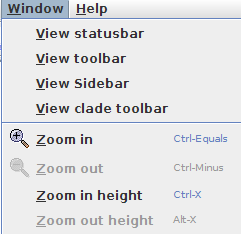
\includegraphics[width=4cm]{menuwindow.png}
\captionof{figure}{\label{fig.menuwindow}Window menu}
\end{center}

\noindent
{\tt Window/View Statusbar}: Toggle visibility of status bar\\
{\tt Window/View Toolbar}: Toggle visibility of tool bar at the top\\
{\tt Window/View Sidebar}: Toggle visibility of tool bar at the side\\
{\tt Window/View Clade Toolbar}: Toggle visibility of tool bar at bottom containing clade information\\
{\tt Window/Zoom in}: Enlarge drawing. Note that this has an impact on the resolution when
exporting bitmap images.\\
{\tt Window/Zoom out}: Draw smaller image.\\
{\tt Window/Zoom in height}: Enlarge drawing, but only in the direction of the tree branch heights. 
Again, this has an impact on the resolution when exporting bitmap images.\\
{\tt Window/Zoom out height}: Draw smaller branch heights.\\

\begin{center}
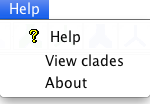
\includegraphics[width=4cm]{menuhelp.png}
\captionof{figure}{\label{fig.menuhelp}Help menu}
\end{center}

\noindent
{\tt Help/Help}: Show short description as shown below.\\
{\tt Help/View Clades}: Show clades in text entry, so the contents can be copied to clipboard.\\
{\tt Help/About}: Show version and citation info.

\begin{center}

\includegraphics[width=\textwidth]{help.png}
\captionof{figure}{\label{fig.help}Show help and other useful information}
\end{center}

\begin{center}
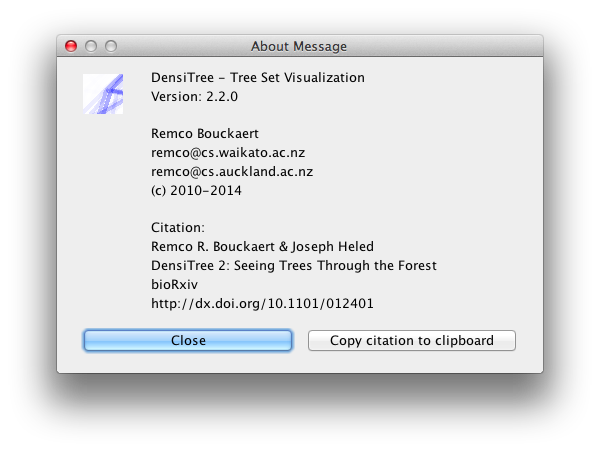
\includegraphics[width=0.5\textwidth]{about.png}
\captionof{figure}{\label{fig.about}Show version and citation information}
\end{center}

\subsection{Toolbar}
The toolbar (
\includegraphics[width=7cm]{toolbar.png}) has the following functions:\\
%\includegraphics[width=5cm,viewport=400 200 600 500,clip]{mcc.png}

\includegraphics[width=8mm,viewport=0 0 28 28,clip]{toolbar.png} open file,\\

\includegraphics[width=8mm,viewport=28 0 52 28,clip]{toolbar.png} draw all,\\

\includegraphics[width=8mm,viewport=52 0 79 28,clip]{toolbar.png} browse to first consensus tree,\\

\includegraphics[width=8mm,viewport=79 0 105 28,clip]{toolbar.png} browse to previous consensus tree,\\

\includegraphics[width=8mm,viewport=105 0 129 28,clip]{toolbar.png} start animation,\\

\includegraphics[width=8mm,viewport=129 0 155 28,clip]{toolbar.png} browse to next consensus tree,\\

\includegraphics[width=8mm,viewport=155 0 182 28,clip]{toolbar.png} browse to last consensus tree,\\

\includegraphics[width=8mm,viewport=182 0 211 28,clip]{toolbar.png} 

\includegraphics[width=8mm,viewport=211 0 237 28,clip]{toolbar.png} increase/decrease tree intensity.\\
\includegraphics[width=8mm,viewport=237 0 265 28,clip]{toolbar.png} 
\includegraphics[width=8mm,viewport=265 0 290 28,clip]{toolbar.png} increase/decrease consensus tree intensity.\\
\includegraphics[width=8mm,viewport=290 0 320 28,clip]{toolbar.png} 
\includegraphics[width=8mm,viewport=320 0 345 28,clip]{toolbar.png} increase/decrease tree line width.\\
\includegraphics[width=16mm,viewport=345 0 398 28,clip]{toolbar.png} increase/decrease consensus tree line width.\\
\includegraphics[width=16mm,viewport=398 0 448 28,clip]{toolbar.png} decrease/increase animation time delay - shorter delay = faster animation.\\
\includegraphics[width=16mm,viewport=448 0 495 28,clip]{toolbar.png} decrease/increase jitter on trees (not consensus trees).\\
and\\
\includegraphics[width=8mm,viewport=495 0 525 28,clip]{toolbar.png} show short help and status.\\

The tool bar can be hidden or made visible again using the {\tt Window/View Toolbar} menu.

\subsection{Sidebar}
The sidebar is by default shown at the right side of the window, but can be dragged to another place.
It contains the following functions:

\includegraphics[width=2.0cm]{\webdir/modedefault.png} Place nodes in the middle of the top of its two child clades.\\
\includegraphics[width=2.0cm]{\webdir/modestar.png} Position nodes as star tree.\\
\includegraphics[width=2.0cm]{\webdir/modecentralised.png} Position nodes halfway the utmost left and utmost right taxon in the clade.\\
\includegraphics[width=2.0cm]{\webdir/modeanglecorrected.png} As above, but put clades at same position as its parent thus forming nodes with more than two child clades.\\

\includegraphics[width=2.0cm]{\webdir/stylestraight.png} draw as triangle tree.\\
\includegraphics[width=2.0cm]{\webdir/styleblock.png} draw as block tree.\\
\includegraphics[width=2.0cm]{\webdir/stylearced.png} draw with arcs.\\
\includegraphics[width=2.0cm]{\webdir/stylesteep.png} draw with steep arcs.\\

The side bar can be hidden or made visible again using the {\tt Window/View Sidebar} menu.

\input{panels.tex}

\subsection{Clade toolbar}

The clade toolbar at the bottom of the screen lists clades sorted by support in the tree set.
When 'view clades' is set to true, clades can be selected in the list, and the
selection changes. Also, when a clade is selected in the tree set by dragging it
in a rectangle, the selected clades are highlighted in the list.

The clade toolbar can be hidden or made visible again using the {\tt Window/View Clade Toolbar} menu.

\subsection{Statusbar}

The main function of the status bar at the bottom of the screen is to show the progress
when drawing all trees and to show the number of the topology when browsing through
the consensus trees.

When the mouse is moved, the height at the mouse position is displayed in the status bar.

When all trees are drawn, the numbers in the status bar count down to zero. When also
consensus trees are drawn, the count goes up. When drawing is complete, the message 
'Done Drawing Trees' appears in the status bar.

The status bar can be hidden or made visible again using the {\tt Window/View Statusbar} menu.

\if0 % these are grossly out of data
\newpage
\subsection{Key short cuts}
\begin{center}
\begin{tabular}{|c|l|}
\hline
Ctrl-O & Open file for reading \\
Ctrl-S & Save tree set\\
Ctrl-P & Print \\
\hline
Ctrl-Z & Undo ordering \\
Ctrl-Y & Redo ordering \\
Ctrl-A & Select all labels \\
Ctrl-U & Unselect all labels \\
Ctrl-M & Move selected labels up \\
M & Move selected labels down \\
\hline 
S, 1 to 6 & Various taxon ordering methods \\
7,8,9 & Use meta data on a tree to position nodes\\
\hline
R & Redraw complete tree set \\
\hline
P & Browse to previous tree in tree set \\
N & Browse to next tree in tree set\\
Ctrl-D & Start animation from current tree\\
\hline
c/Ctrl-c &decrease/increase consensus tree intensity\\
i/Ctrl-i &decrease/increase tree intensity\\
j/Ctrl-j &decrease/increase jitter on trees (not consensus trees)\\
w/Ctrl-w &decrease/increase consensus tree line width\\
v/Ctrl-v &decrease/increase tree line width\\
f/Ctrl-f &decrease/increase animation time delay - shorter delay = faster animation\\
t/Ctrl-t &decrease/increase number of drawing threads for drawing tree set\\
n/Ctrl-n &decrease/increase threshold for angle correction\\
\hline
+ & Zoom in \\
- & Zoom out \\
H/Ctrl-H &zoom in/out tree height\\
\hline
Alt-F & show File menu\\
Alt-E & show Edit menu\\
Alt-D & show Draw all menu\\
Alt-B & show Browse menu\\
Alt-S & show Settings menu\\
Alt-W & show Window menu\\
Alt-H & show Help\\
\hline
\end{tabular}
\captionof{table}{Key shortcuts}
\end{center}
\fi

\newpage
\section{FAQ\label{sec.faq}}

\subsection{How do I move leafs?}

This depends on the tree type. For default and centralised trees, first you select the leafs that you want to move.
You can select leafs by clicking on them individually, or by dragging a rectangle
over the set of leafs you want to select. By keeping the shift key pressed, the
selection can be added to. By keeping the control key pressed, any leaf that is
selected will be toggled from the selection. Once the appropriate set of leafs
is selected, press M to move down and control-M to move in the other direction.

Furthermore, for star trees you can enable show clades. Circles appear on the taxa,
which you can select by clicking on it, or drag a rectangle over it. The selection
can be dragged. This allows you to position the taxa at irregular intervals.


\subsection{I'm loading a large file, but nothing seem to happen?!?}

If nothing happens after a few minutes, most likely it is java that has run out
of memory. To start \DensiTree\ with access to more memory, start it from the 
command line with

\begin{verbatim}java -Xmx3g -jar DensiTree.jar\end{verbatim}

Here '3g' means 3 gigabyte. If you need even more, change the 3 to a higher number.


\subsection{How do I start \DensiTree\ with my favorite settings?}
First, find out the values of the current settings. This can be done
using the Help/Help menu, which makes a dialog pop up that shows the
current status. At the bottom, it also shows how to start up \DensiTree\ 
with these settings from the command line.


\subsection{How do I specify burn in?}
Start \DensiTree\ from the command line with the -b option, e.g. using\\
{\tt java -jar DensiTree.jar -b 100}\\
This will skip the first 100 trees every time a nexus tree is read.
To check current burn in, select the Help/Help menu. The dialog shows
the current state.

\subsection{What does the color coding mean?}
The most popular tree is blue, the next most popular red, the third most
popular green and the rest is dark green.

Consensus trees are blue by default as are labels. Height bar and grid
are black by default.

\subsection{How do I change these colors?}
Colors can be changed using the Settings/Set Color submenu.
To start \DensiTree\ with specific colors, colors can be specified from the command line 
or via a script as follows:\\
{\tt java -Dcolor.1=0x000000 -jar DensiTree.jar}\\
sets the color of the most popular tree to black.
The part 'color.1' specifies that it is the most popular color,
and 0X000000 specifies the RGB value in hexadecimal.

The current color settings can be found using the Help/Help menu, where they
are shown near the bottom of the dialog that pops up then.

The following colors can be specified that way:\\
{\tt color.1} for most popular topology,\\
{\tt color.2} for next most  popular topology,\\
{\tt color.3} for third most popular topology,\\
{\tt color.default} for remainder of topologies,\\
{\tt color.cons} for consensus trees,\\
{\tt color.label} for color of labels,\\
{\tt color.height} for color of height grid and height bar,\\
{\tt color.bg} for back ground color.\\
{\tt color.rootcanal} for root canal color.

So, to make consensus trees red and labels black, you start
\DensiTree\ like this:\\
{\tt java -Dcolor.cons=0xFF0000 -Dcolor.label=0X000000 -jar DensiTree.jar}\\

\subsection{How do I change the label font?}
Use the Settings/Set Font menu.

\subsection{Can I batch process tree set files?}
Use the command line options to specify your settings, and use the 
\begin{verbatim}-o <filename>\end{verbatim} option to specify a file.
The DensiTree is exported as png file to the specified file.

\subsection{My tree is a mess, what do I do?}

Check that you have a clock like tree. DensiTree may work for non-clock like trees, but
was not designed to do so. Otherwise, try one of the tricks in the next question.

\subsection{My tree has many crossing lines, what do I do?}
\noindent o Step 1: Try the reshuffle using the Edit/Shuffle menu and try the various methods.
Most methods work on some tree sets, but none work for all.

\noindent o Step 2: If the tree looks half decent, use the tree editor to rotate parts of the
tree. You can show the tree editor using the Edit/Show Tree Edit menu. To rotate part of the
tree, click on an icon at an internal node.

\noindent o Step 3: The location of internal nodes can be changed by dragging them with
the right mouse button. This can help getting rid of some crossing branches.

\subsection{How can I visualise meta data?}

When there is meta data on the branches, such as populations sizes, branch rates or migration rates,
DensiTree can be used in two ways to visualise this meta data.

1. By positioning all internal nodes at the height that the meta data value indicates.
Press 7, 8 or 9 to get such a tree. The difference between the methods is that
7 shows the meta data values for each individual branch, 8 shows the mean meta data value
at a particular height in the tree and 9 shows the sum of the meta data values.

2. By drawing lines with a width proportional to the meta data value.

\subsection{How can I specify which meta data is used?}

The simplest way is when you know in which order the metadata is inserted in the tree set file.
Say, meta data is of the form \begin{verbatim}[&rate=0.1234,popsize={13.31, 11.01}]\end{verbatim}
then there are three numbers: one for rate, and two fro popsize. To make the bottom of a branch
equal to the rate, we need the first number. With menu settings/meta data/Bottom pattern number,
a dialog pops up where you can enter '1' for the rate, '2' for the first popsize, and '3' for
the last pop size.

For experts, under menu settings/meta data/pattern, you can specify a regular expression that will be matched
with the meta data in the tree file. This pattern will be used by both methods of meta data
visualisation.

\subsection{How can I specify which meta data is used for the bottom and top of a line?}

With menu settings/meta data/Top pattern number, you can specify the number in the meta data.
Note that the top of a branch need to be before the bottom of a branch.

Also, for experts, as in the previous question, but define two groups in the regular expression.
The first group is used at the bottom of the branch and the second group at the top.

\subsection{How do I create a phylogeographical DensiTree?}
o Step 1: load a tree set file (Menu File/load)

\noindent o Step 2: load geographical locations (Menu File/Load geographic) encoded in a KML or KMZ file as
produced in Google earth.

\noindent o Step 3: load a bitmap image (Menu File/Background image) with a world map.
Alternatively, load a file of a map in Mercator projection which has the 
corners of the rectangle covered by the image encoded in its file name (see 
description of File/Background image for details).

\subsection{The labels get all mixed up when the root is at the top. What do I do?}
Rotate labels, using the Settings/Rotate labels menu. This only has an effect when the root
is drawn at the top.


%\subsection{How do I cite DensiTree in a publication?}
%
%Remco R. Bouckaert\\
%DensiTree: making sense of sets of phylogenetic trees\\
%Bioinformatics (2010) 26 (10): 1372-1373.\\
%doi: 10.1093/bioinformatics/btq110


\newpage
\section{Command line options\label{sec.cmd}}

Starting \DensiTree\ from the command line or from a script allows
one to customize default settings. \DensiTree\ is started using
\begin{verbatim} 
java [vmoptions] -jar DensiTree [options] [file]
\end{verbatim}
The following options can be used:
\begin{verbatim} -c <float nr>\end{verbatim}
 intensity used for drawing consensus trees, default 1
\begin{verbatim}-i <float nr>\end{verbatim}
 intensity used for drawing trees, default 1
\begin{verbatim}-j <int nr>\end{verbatim}
jitter used for drawing x-position of nodes, default 0
\begin{verbatim}-w <int nr>\end{verbatim}
width of consensus tree lines, default 4
\begin{verbatim}-v <int nr>\end{verbatim}
width of tree lines, default 1
\begin{verbatim}-f <int nr>\end{verbatim}
delay between drawing two frames in animation in milliseconds, default 100
\begin{verbatim}-t <int nr>\end{verbatim}
number of threads used for drawing tree set, default 2
\begin{verbatim}-b <int nr>\end{verbatim}
burn in, i.e., the number of trees at the start of the tree set that are ignored, default 0. NB this is not the number of samples in
the MCMC run that are ignored, but the actual number of trees.
\begin{verbatim}-scalemode [none|short|full]\end{verbatim}
set the grid. Should be one of 'none' for no grid (default), 'short' to show a scale or 'full' to show lines throughout image
\begin{verbatim}-li <float nr>\end{verbatim}
sets up label indent, default 0
\begin{verbatim}-o <file>\end{verbatim}
sets output file. The tree set specified through the command line is drawn and
exported in png format to the specified file name. 
This can be useful for batch image processing.
\begin{verbatim}-KML <File name>\end{verbatim}
KML file with geographical locations
\begin{verbatim}-geowidth <int nr>\end{verbatim}
widht of the link between taxon and its geographical location
\begin{verbatim}-geocolor <color>\end{verbatim}
color of the link between taxon and its geographical location
\begin{verbatim}-bg <file>\end{verbatim}
sets the background image
\begin{verbatim}-bd <BranchDrawer class>\end{verbatim}
sets the method for drawing branches. Available methods are
"viz.graphics.BranchDrawer" for lines (default),
"viz.graphics.ArcBranchDrawer" for arcs, and
"viz.graphics.SteepArcBranchDrawer" for steep arcs.
\begin{verbatim}-pattern <pattern>\end{verbatim}
specifies meta data pattern. Useful for drawing trees with one of the
shuffle options using meta data. A regular expression pattern should be
specified following the java conventions (see for example
\url{http://download.oracle.com/javase/1.4.2/docs/api/java/util/regex/Pattern.html})
which matches the complete meta data annotation in the tree.
\begin{verbatim}-colorpattern <pattern>\end{verbatim}
Colors taxon labels differently where the color is selected randomly.
A group needs to be defined in the regular expression.
Every taxon matching the same part in this group gets the same color.
For example \begin{verbatim} -colopattern ^(..).*$\end{verbatim} makes all taxa with the same
two starting letters the same color.
\begin{verbatim}-rotatetext\end{verbatim}
to rotate labels when the root is drawn at the top.
\begin{verbatim}-singlechild\end{verbatim}
allow parsing files with nodes that have single child instead of two children.



If a file is specified, it should be after the last option. \DensiTree\ will attempt
to open that file on start up.

The following virtual machine options ({\tt [vmoptions]} above) can be useful:\\
{\tt -Dcolor.1=0XFF0022} to specify color of most popular topology,\\
{\tt -Dcolor.2=0XFF0022} for next most  popular topology,\\
{\tt -Dcolor.3=0XFF0022} for third most popular topology,\\
{\tt -Dcolor.default=0XFF0022} for remainder of topologies,\\
{\tt -Dcolor.cons=0XFF0022} for consensus trees,\\
{\tt -Dcolor.label=0XFF0022} for color of labels,\\
{\tt -Dcolor.height=0XFF0022} for color of height grid and height bar,\\
{\tt -Dcolor.bg=0XFF0022} for back ground color.

The color is specified as RGB color in Hexadecimal (the number 0XFF0022 listed
in all options above).


\newpage
\section{Acknowledgements}

Joseph Heled's enthusiasm, bug reports and suggestions helped a lot in improving
\DensiTree\ in a short period of time. Furthermore, he made tree sets available for
improving the gallery in this document. Simon Greenhill kindly made tree sets available 
for the gallery.

\bibliographystyle{plain}
\begin{thebibliography}{1}
\bibitem{BEAST}
Bouckaert RR, Heled J, Kuehnert D, Vaughan TG, Wu C-H, Xie D, Suchard MA,
Rambaut A, Drummond AJ (2014) BEAST 2: A software platform for Bayesian
evolutionary analysis. PLoS Computational Biology 10(4): e1003537
\bibitem{FigTree}FigTree. Andrew Rambaut
\url{http://tree.bio.ed.ac.uk/software/figtree/}
\bibitem{SplitsTree}D. H. Huson and D. Bryant, Application of Phylogenetic Networks in Evolutionary Studies, Mol. Biol. Evol., 23(2):254-267, 2006.
\url{http://www.splitstree.org/}
\bibitem{poly}
Greenhill, S.J., Blust. R, Gray, R.D. The Austronesian Basic Vocabulary Database: From Bioinformatics to Lexomics. Evolutionary Bioinformatics, 4:271-283. 2008.
\bibitem{treeviz}
Nina Amenta, Jeff Klingner.
Case Study: Visualizing Sets of Evolutionary Trees.
University of Texas at Austin.
2002 IEEE Symposium on Information Visualization (InfoVis), pp.71, 2002.
\bibitem{treeviz2}
Hillis, D.M., T.A. Heath, and K. St. John.
Analysis and Visualization of Tree Space. 
Systematic Biology 54(3):471-82, Jun 2005.
\bibitem{maddison}
Maddison, D. R. 
The discovery and importance of multiple islands of most-parsimonious trees. 
Syst. Zool. 40:315–328. 1991
\bibitem{mrbayes}
Huelsenbeck, J. P., F. Ronquist, R. Nielsen and J. P. Bollback. 2001. Bayesian inference of phylogeny and its impact on evolutionary biology. Science 294: 2310-2314.
\url{http://mrbayes.csit.fsu.edu/}
\end{thebibliography}


\end{document}
